\section{Methods}

\subsection{Integrative-microbiomics, a webtool}
\begin{figure*}[h]
	\centering
	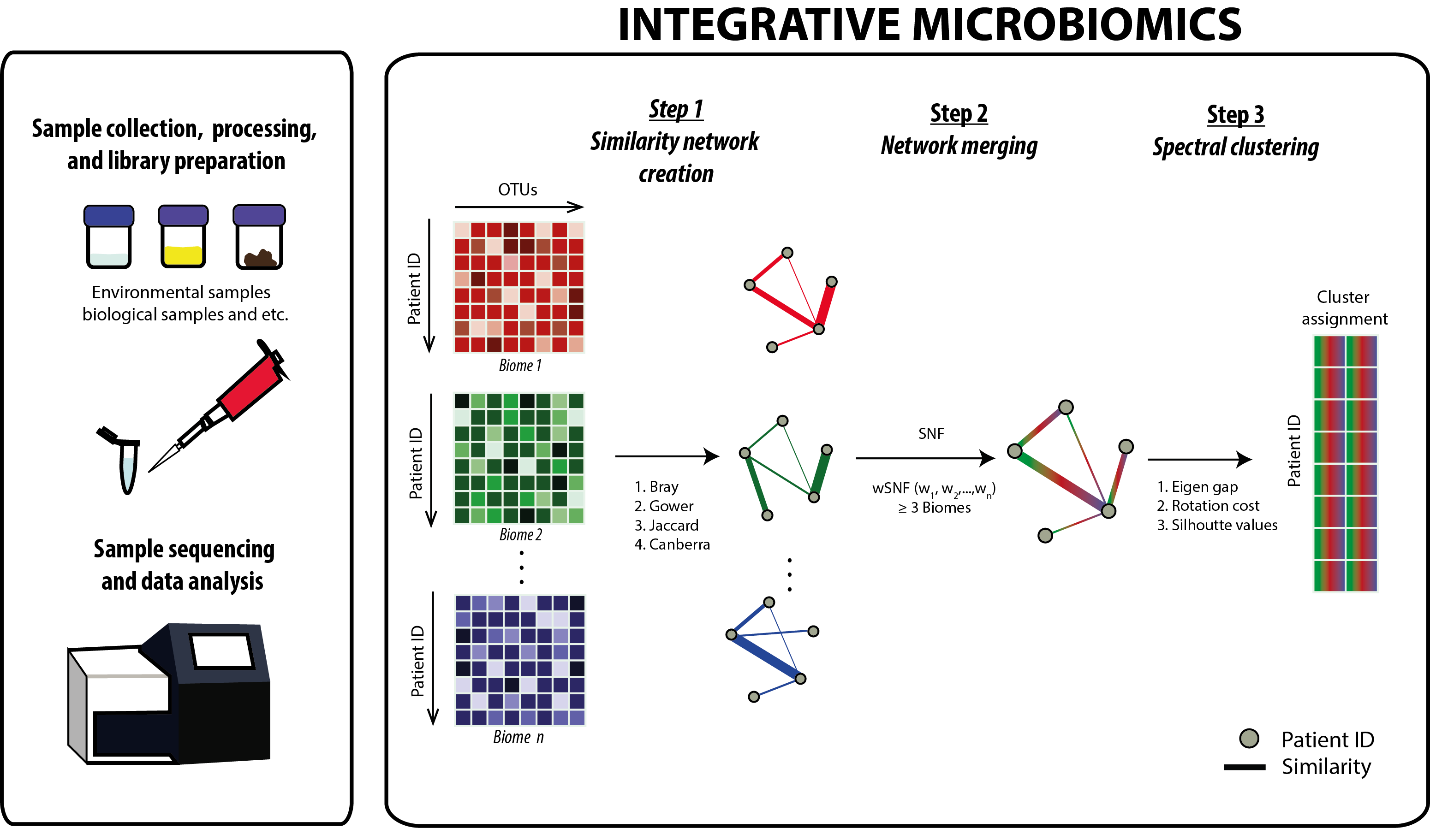
\includegraphics[width=\textwidth]{image/webtool_intro.png}
	\caption{A figure describing the workflow of integrative microbiomics. The input microbiome datasets, are converted into patient/sample similarity networks based on the user-specified similarity measures: 1) Bray-Curtis, 2) Gower, 3) Canberra and 4) Jaccard; before merging them using the user-specified algorithm: 1) SNF, 2) wSNF. Further, the tool then implements a spectral clustering algorithm to allow cluster analysis on the merged dataset.}
	\label{fig3}
\end{figure*}

Given the input microbiome datasets, the tool converts them into patient/sample similarity networks for each view based on the user-specified similarity measure before merging them using the user-specified algorithm. Further, the tool then implements a spectral clustering algorithm to allow cluster analysis on the merged dataset outputting the cluster assignments for each sample/patient. The optimum default number of clusters is computed using ensemble-based voting of three differing methodologies: Best Eigen Gap, Rotation cost and average silhouette method (Figure\ref{fig3}). For a given value of `k' (the number of clusters), we calculate a score/vote using the below rules

\begin{enumerate}
	\item If the average silhouette score > 0.7 $\rightarrow$ Score = Score + 3
	\item If 0.5 < average silhouette score < 0.7 $\rightarrow$ Score = Score + 2
	\item If 0.3 < average silhouette score < 0.5 $\rightarrow$ Score = Score + 1
	\item If k equals the first best value as derived from eigen gap method $\rightarrow$ Score = Score + 3
	\item If k equals the second-best value as derived from eigen gap method $\rightarrow$ Score = Score + 2
	\item If k equals the first best value as derived from rotation cost method $\rightarrow$ Score = Score + 3
	\item If k equals the second-best value as derived from rotation cost method $\rightarrow$ Score = Score + 2 
\end{enumerate} 
The value of k for which the Score is the highest is chosen as the default optimum number of clusters. In addition, the tool also outputs the integrated similarity matrix which can be used for downstream analysis such as for label propagation and survival analysis \cite{Wang2014}.

The tool presently provides four similarity measures 1) Bray-Curtis, 2) Gower, 3) Canberra and 4) Jaccard, appropriate for microbiome datasets which is used to construct patient/sample similarity network and two approaches 1) SNF, 2) wSNF to integrate these networks. For the implementation of wSNF the following formula in SNF
$$P^{(v)}=S^{(v)} \times \frac{\sum_{k=v} p^{k}}{(m-1)} \times (S^{(v)})^{T}, v=1,2,3, \ldots, m$$ was modified into $$P^{(v)}=S^{(v)} \times \frac{\sum_{k=v} \omega_{k} \times p^{(k)}}{\sum_{k \neq v} \omega_{k}} \times(S^{(v)})$$ $v=1,2,3, \ldots, m$
where $\omega_{k}$ is the weight of the $k^{ th}$ dataset, $m$ the total number of views, $P$ the status matrix and $S$ the kernel matrix as defined by Wang et.al \cite{Wang2014}.

This webtool allows the users to integrate multiple microbiome datasets obtained from different sites in a patient/biological entity or from various methods (targeted sequencing, metagenomics and qPCR) from the same site. For example, the lung microbiome (bacteria) with the gut microbiome (bacteria) or the lung microbiome (bacteria) with lung mycobiome. The tool assumes each input microbiome datasets represent a view of an underlying biological mechanism or a disease. Reliable estimation of each view is assumed when using SNF \cite{Jiang2019}. However, it may not be always practical to reliably estimate each view, although they play an equal role in the underlying biological process. This is due to the limitations and differing rates of development, in the present technologies and reference databases. In such cases, a weighted SNF approach is preferred, which still assumes the input datasets share an underlying biological mechanism but accounts for inconsistency of the microbiome data based on the user specified weights. The default weights are assigned based on the taxonomical richness (i.e. the number of microbes present) of the datasets. 

The interface of the webtool was developed using Rshiny and is available through Shiny Server (Open Source) in confluence with nginx-1.19.1. The tool is powered by custom scripts written in python2.7 and R; and containerized using Docker for ease of offline implementation. The developed webtool can be accessed at \url{https://integrative-microbiomics.ntu.edu.sg}.

\subsection{Longitudinal assessment of Exacerbation}

A longitudinal cohort of n=17 patients were recruited from two hospitals in the east of Scotland (2016-2017) to study changes in the microbiome during exacerbation and following antibiotic treatment. DNA and RNA extraction were performed on sputum samples obtained from each patient and on a blank sterile PBS (Phosphate buffer solution). The extracted DNA was subjected to targeted amplicon sequencing of the 16S rRNA and ITS2 regions of the genome to derive the Microbiome and Mycobiome, by mapping them to green genes and UNITE databases, respectively. Blank samples contained read counts many orders of magnitude lower than test samples and hence unlikely to have any influence on the observed microbiome. RT-qPCR (real time quantitative polymerase chain reaction) was performed on the cDNA derived from the extracted RNA to quantify the viral burden of the 17 viruses investigated in each patient. $\alpha$ and $\beta$ diversity of the multi-biome was calculated from the concatenated microbiome and the integrated patient similarity matrix using the “vegan” package in R.

\subsection{Antibiotic action simulation}

To predict the impact of antibiotics on the interactome, $\beta$-lactam antibiotic action was simulated by a 75\% reduction in the relative abundance of the microbes targeted by this antibiotic in the baseline (pre-antibiotic) state including the following genera: \emph{Streptococcus, Staphylococcus, Haemophilus, Moraxella, Actinomyces, Arachnia, Bacteroides, Bifidobacterium, Eubacterium, Fusobacterium, Lactobacillus, Leptotrichia, Peptococcus, Peptostreptococcus, Propionibacterium, Selenomonas, Treponema and Veillonella}. In order to remove interactions resulting from random noise at the expense of sensitivity to weak signals and to allow comparison between the derived interactomes, the following abundance and prevalence filters were applied followed by co-occurrence analysis; retention of microbes present at greater than 1\% abundance in at least three subjects; in the pre OR post OR modelled antibiotic state.

\subsection{``Time to next exacerbation" prediction}

To predict “Time to next exacerbation”, Microbiome datasets were CLR (Centred log ratio) transformed before concatenation and microbes that are present in at least 4 patients at an abundance of 1\% were considered for further analysis. To derive pairwise microbial interactions for each patient, LIONESS \cite{Kuijjer2019}, a single patient network inference framework was implemented with General Boosted Linear model (GBLM) as the network inference algorithm. Correlation between the abundance of each microbes and interaction strength with ‘time to next exacerbation’ was assessed using Spearman’s rank correlation with statistical testing. Multivariate adaptive regression spline (MARS) \cite{Friedman1991}, a non-linear regression model was implemented with microbes or interaction strength as the predictor variable to predict ‘time to next exacerbation’ groups; defined as (Time to exacerbation: $<$12 weeks and $>$12weeks). The goodness of the fit of the model was evaluated by computing the R-squared (RSq) and the Generalized R-squared metric (GRsq). A feature importance plot based on Generalized Cross validation score (gcv) was also computed on the feature selected (microbes) by the model.  All the above analysis was implemented in R using the following packages 1)”Hmisc” 2) “earth” 3)”vegan” 4)”compositions” 5)”lionessR”.

\subsection{Validation of the interactome}

Experimental microbiological validation of Pseudomonas aeruginosa and Aspergillus fumigatus interaction was performed using one strain Aspergillus fumigatus (Af293) and three strains of Pseudomonas aeruginosa: (1) lab strain (PAO1) as control and (2,3) two clinical isolates of Pseudomonas aeruginosa derived from “low-risk” and “high-risk” patient clusters. The interaction was investigated using the disk inhibition method as described by Homa et al. \cite{Homa2019}.
An independent cohort of 166 patients was recruited from 4 sites (3 in Singapore and 1 in Dundee, Scotland) to validate the high-risk cluster and its interactome. DNA extraction was performed on the collected sputum samples of each patient. A shotgun metagenomic sequencing was performed at the NTU core sequencing facility on these samples according to the methods described by Gusareva et al. \cite{Gusareva2019}. Kaiju \cite{Menzel2016} with default parameters was implemented on the raw sequences after human read removal to estimate the taxonomic composition by referencing against NCBI BLAST nr+euk database. Estimation of the viruses that include prokaryotic phages and eukaryotic viruses was implemented using a custom pipeline that uses Demovir (\url{https://github.com/feargalr/Demovir}).